 \subsection{Bah\'ia rectangular de ancho unitario}
  Para validar los resultados de la implementaci\'on del algoritmo, y estudiar la convergencia de \'este, se ha escogido una soluci\'on anl\'itica al problema presentado en la ecuaci\'on \eqref{helmholtz}. Este caso corresponde a una bah\'ia cuadrada de largo unitario cuyo interior es $\Omega = [0,1]\times[0,1]$, la cual se encuentra cerrada por bordes impermeables, es decir, $\partial \Omega_g=0$, y fondo a profundidd $h_0\in\mathbb{R^+}$. Por medio de separaci\'on de variables, al asumir que $u$ puede escribirse como $u(x,y)=f(x)g(y)$, y al considerar las condiciones de borde, se deduce que los modos de oscilaci\'on vienen dados por 
  
  \begin{equation}
    \begin{array}{cc}
    u_{nm}(x,y)=A_{nm}\cos(n\pi x)\cos(m\pi y) & \text{ con } n,m \in \mathbb{N}_0 \text{ y } A_{nm}\in\mathbb{R}
    \end{array}
    \label{eq:bahia_cerrada_modo}
  \end{equation}

  y el per\'iodo de oscilaci\'on asociado
  
  \begin{equation}
    \begin{array}{cc}
    T_{nm}=\dfrac{2}{\sqrt{gh}}\left( n^2+m^2\right)^{-1/2} & \text{ con } n,m \in \mathbb{N}_0
    \end{array}
    \label{eq:bahia_cerrada_periodo}
  \end{equation}

La soluci\'on mediante FEM es implementada para distintas resoluciones de malla y analizada su convergencia mediante la determinaci\'on del error asociado al valor propio y el error asociado al vector propio correspondiente.

Para el caso del error en el valor propio se utilza norma natural de $\mathbb{R}$

$$E = |\lambda^h - \lambda|$$

donde  \hilight{$\lambda$} es la longitud de onda obtenida mediante la soluci\'on anal\'itica \hilight{$\lambda^h$} es la longitud de onda obtenida mediante aproximaci\'on por FEM\\

Para el caso del error en el valor de la desnivelaci\'on superficial el error se calcula mediante la norma de $\mathcal{L}^2(\Omega,\mathbb{R})$

$$E = \left(\int_{\Omega} (u^h - u) \mathrm{d}\boldsymbol{x} \right)^{1/2}$$

Los resultados para el valor propio se muestran en la figura \ref{fig:velores_propios}

\begin{figure}
  \centering
  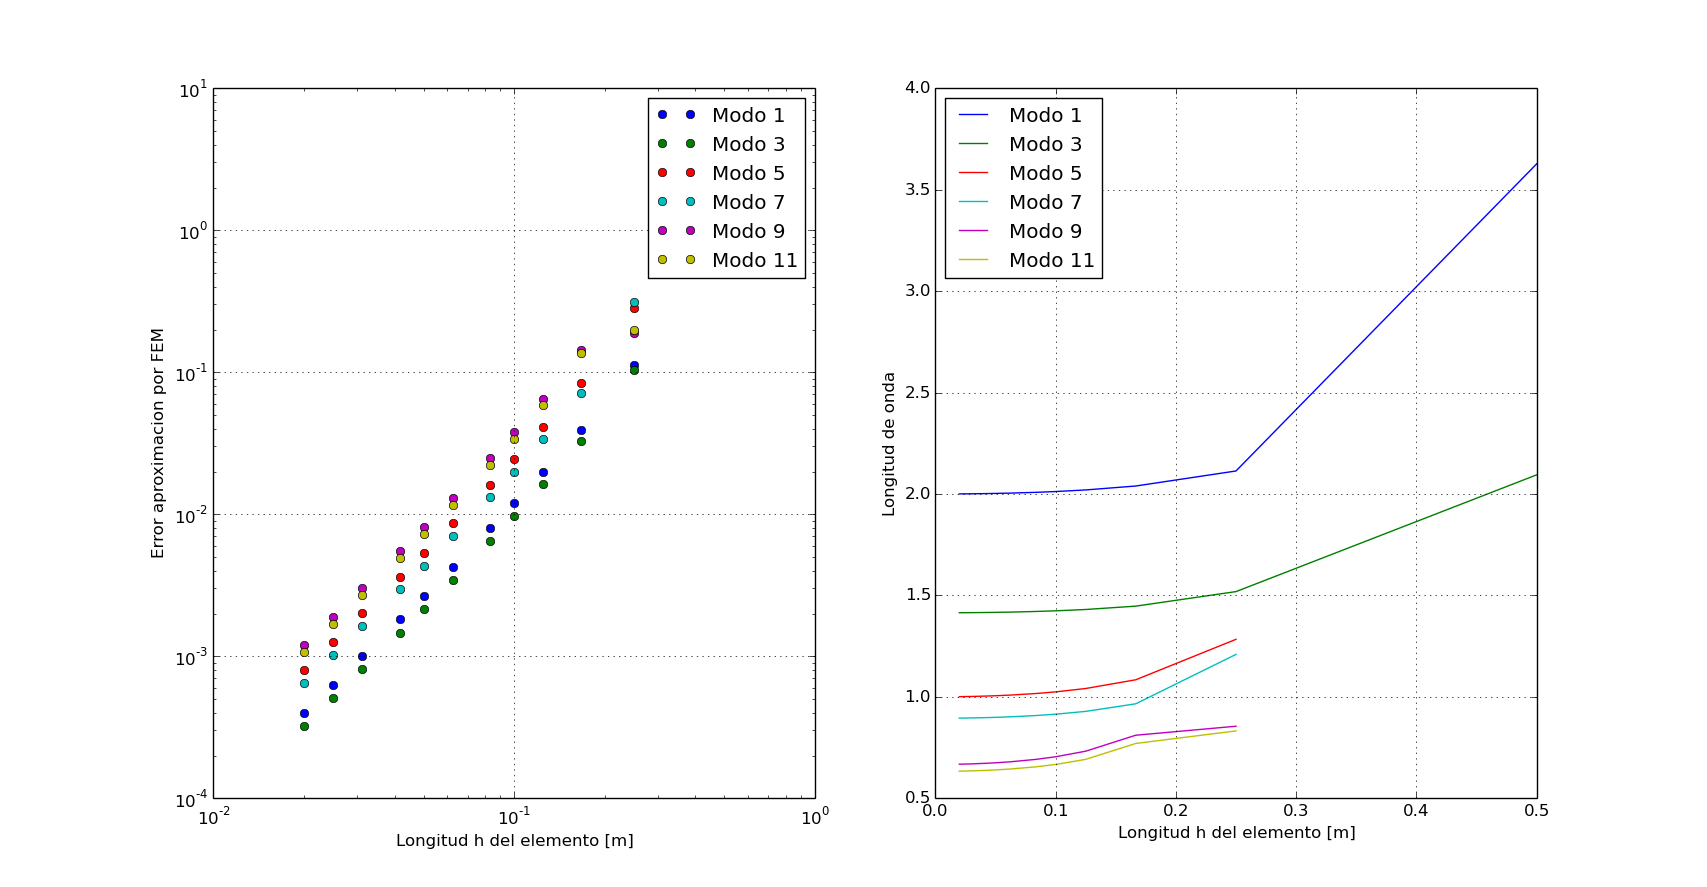
\includegraphics[width=17cm]{figuras/valores_propiosFEM.png}
  \caption{ Resultados aproximaci\'on valores propios mediante FEM y errores asociados}  
  \label{fig:velores_propios}
\end{figure}

Ajustando una curva a los datos ($log(E)$, $log(h)$) se obtiene una recta $log(E) = log(C) + p log(h)$ donde p es la taza de convergencia


\begin{table}[h]
\centering
\begin{tabular}{|c|c|c|}
\hline 
Modo & C & p \\ 
\hline 
1 & 0.62007961 & 2.4403783 \\
\hline 
3 & 0.39830035 & 2.33894099 \\ 
\hline 
5 & 0.69813644 & 2.26494859 \\  
\hline 
7 & 0.71017628 & 2.33846474 \\ 
\hline 
9 & 0.68486822 & 2.12311422 \\  
\hline 
11 &  0.70325574 & 2.17136287 \\
\hline 
\end{tabular} 
\caption{\hilight{Coeficientes de ajuste de las curvas $\log(E_\lambda)=\log(C)+p\log(h)$}}
\end{table}

Para el caso de la convergencia de los \hilight{vectores propios}, los resultados se muestran en la figura \ref{fig:vectores_propios}

\begin{figure}
  \centering
  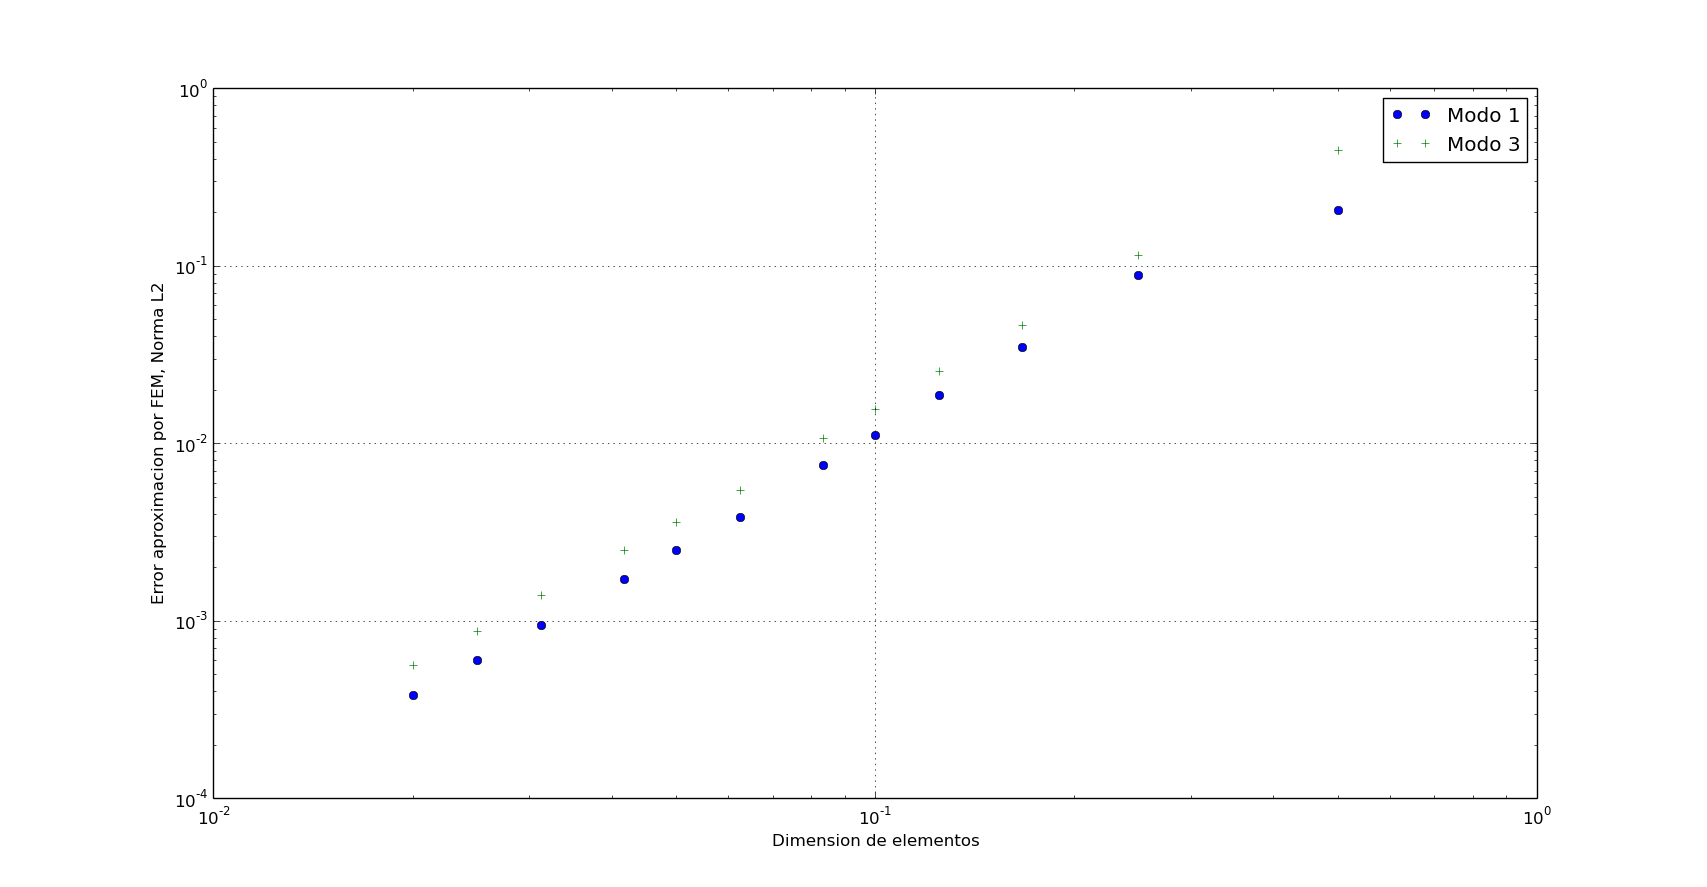
\includegraphics[width=17cm]{figuras/vectores_propiosFEM.png}
  \caption{ \hilight{Errores en norma $\mathcal{L}^2$ de los vectores asociados a cada modo propio}  }
  \label{fig:vectores_propios}
\end{figure}

Ajustando una recta a los datos ($log(E)$, $log(h)$)
\begin{table}[h]
  \centering
  \begin{tabular}{|c|c|c|}
  \hline 
  Modo & C & p \\ 
  \hline 
  1 & 0.0765871 & 2.04894336 \\  
  \hline 
  3 & 0.29036431 & 2.09300275 \\  
  \hline 
  \end{tabular} 
  \caption{\hilight{Coeficientes de ajuste de las curvas $\log(E_u)=\log(C)+p\log(h)$}}
\end{table}

En ambos casos se puede ver que la taza de convergencia es de orden 2.

\begin{figure}
  \centering
  \begin{subfigure}{0.3\textwidth}
    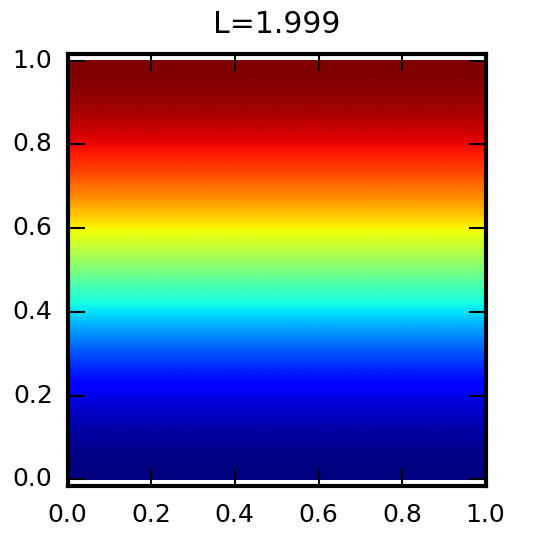
\includegraphics{figuras/modonum_1.png}
  \end{subfigure}
  ~
  \begin{subfigure}{0.3\textwidth}
    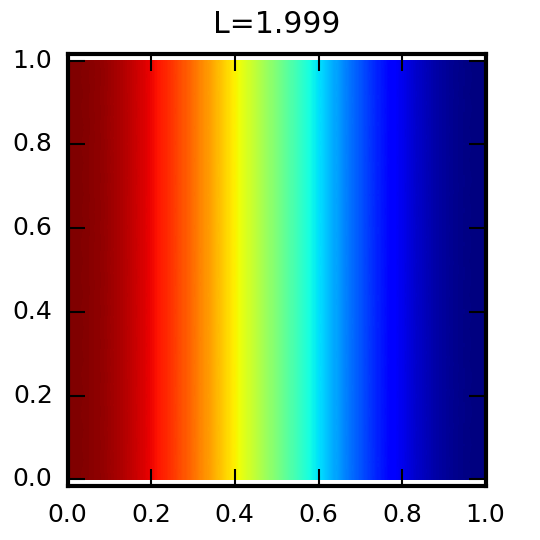
\includegraphics{figuras/modonum_2.png}
  \end{subfigure}
  
  \caption{Modos de oscilaci\'on 1 y 2 usando $h=1/25$ usando el m\'etodo de Elementos Finitos.}
\end{figure}

\begin{figure}  
  \centering
  \begin{subfigure}{0.4\textwidth}
    \centering
    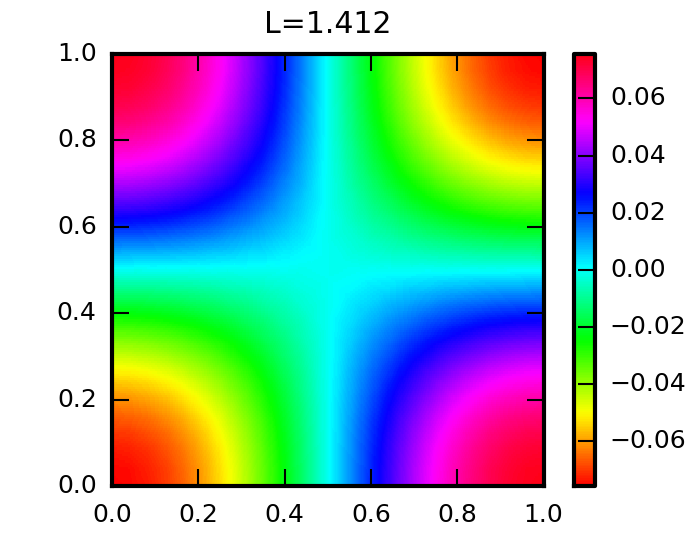
\includegraphics{figuras/modonum_3.png}
  \end{subfigure}
  ~
  \begin{subfigure}{0.4\textwidth}
    \centering
    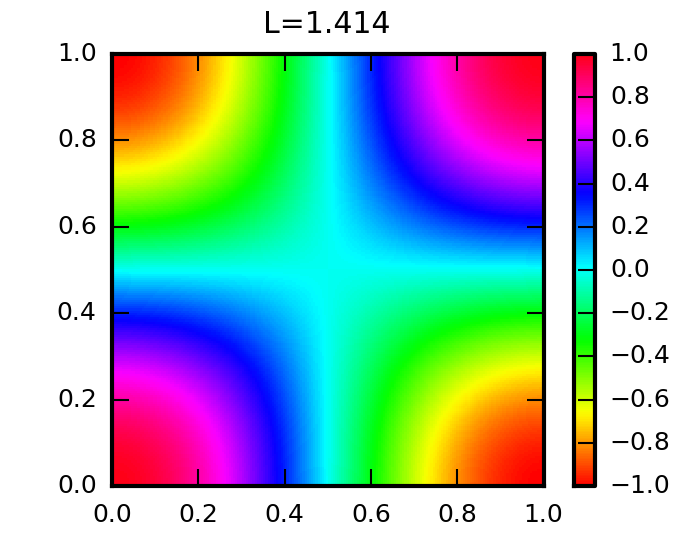
\includegraphics{figuras/modoanalitico_1_1.png}
  \end{subfigure}
  
  
  \begin{subfigure}{0.4\textwidth}
    \centering
    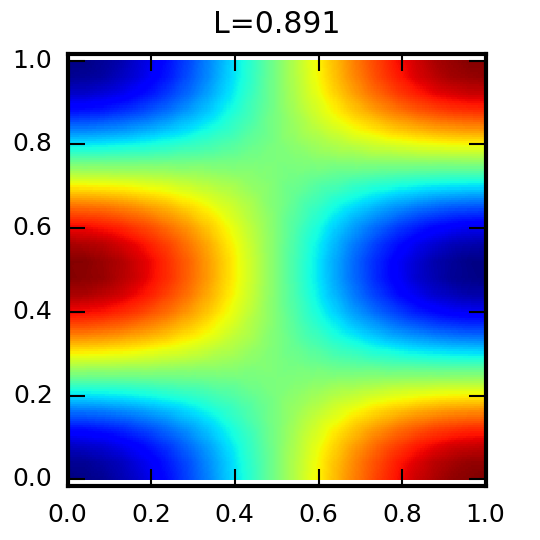
\includegraphics{figuras/modonum_6.png}
  \end{subfigure}
  ~
  \begin{subfigure}{0.4\textwidth}
    \centering
    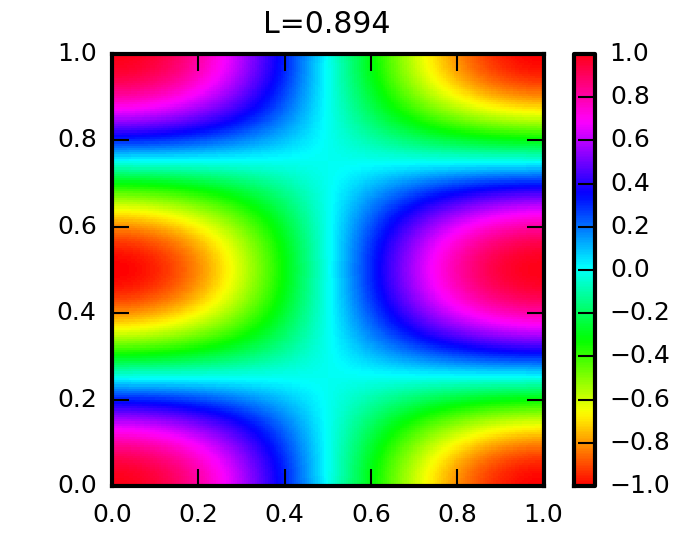
\includegraphics{figuras/modoanalitico_1_2.png}
  \end{subfigure}
  
  \caption{Modos de oscilaci\'on 3 y 6 obtenidos num\'ericamente para $h=1/25$ (primera columna) y mediante la soluci\'on anal\'itica para $(n,m)=(1,1)$ y $(n,m)=(1,2)$ (segunda columna)}
\end{figure}

